\chapter{RESULTADOS}
Foram realizados testes simulando frequências com o gerador de função. Foi simulado uma frequência de 37 Hz, que passou pelos filtros e amplificador, posteriormente processado pelo microcontrolador e enviado ao software, podemos visualizar o sinal na Figura 7 e a Figura 8 demonstra o sinal manipulado com o uso da DFT.

\begin{figure}[htb]
	\caption{Software supervisório - Entrada sinal}
	%	\label{diag:grafico6}
	\borda{
		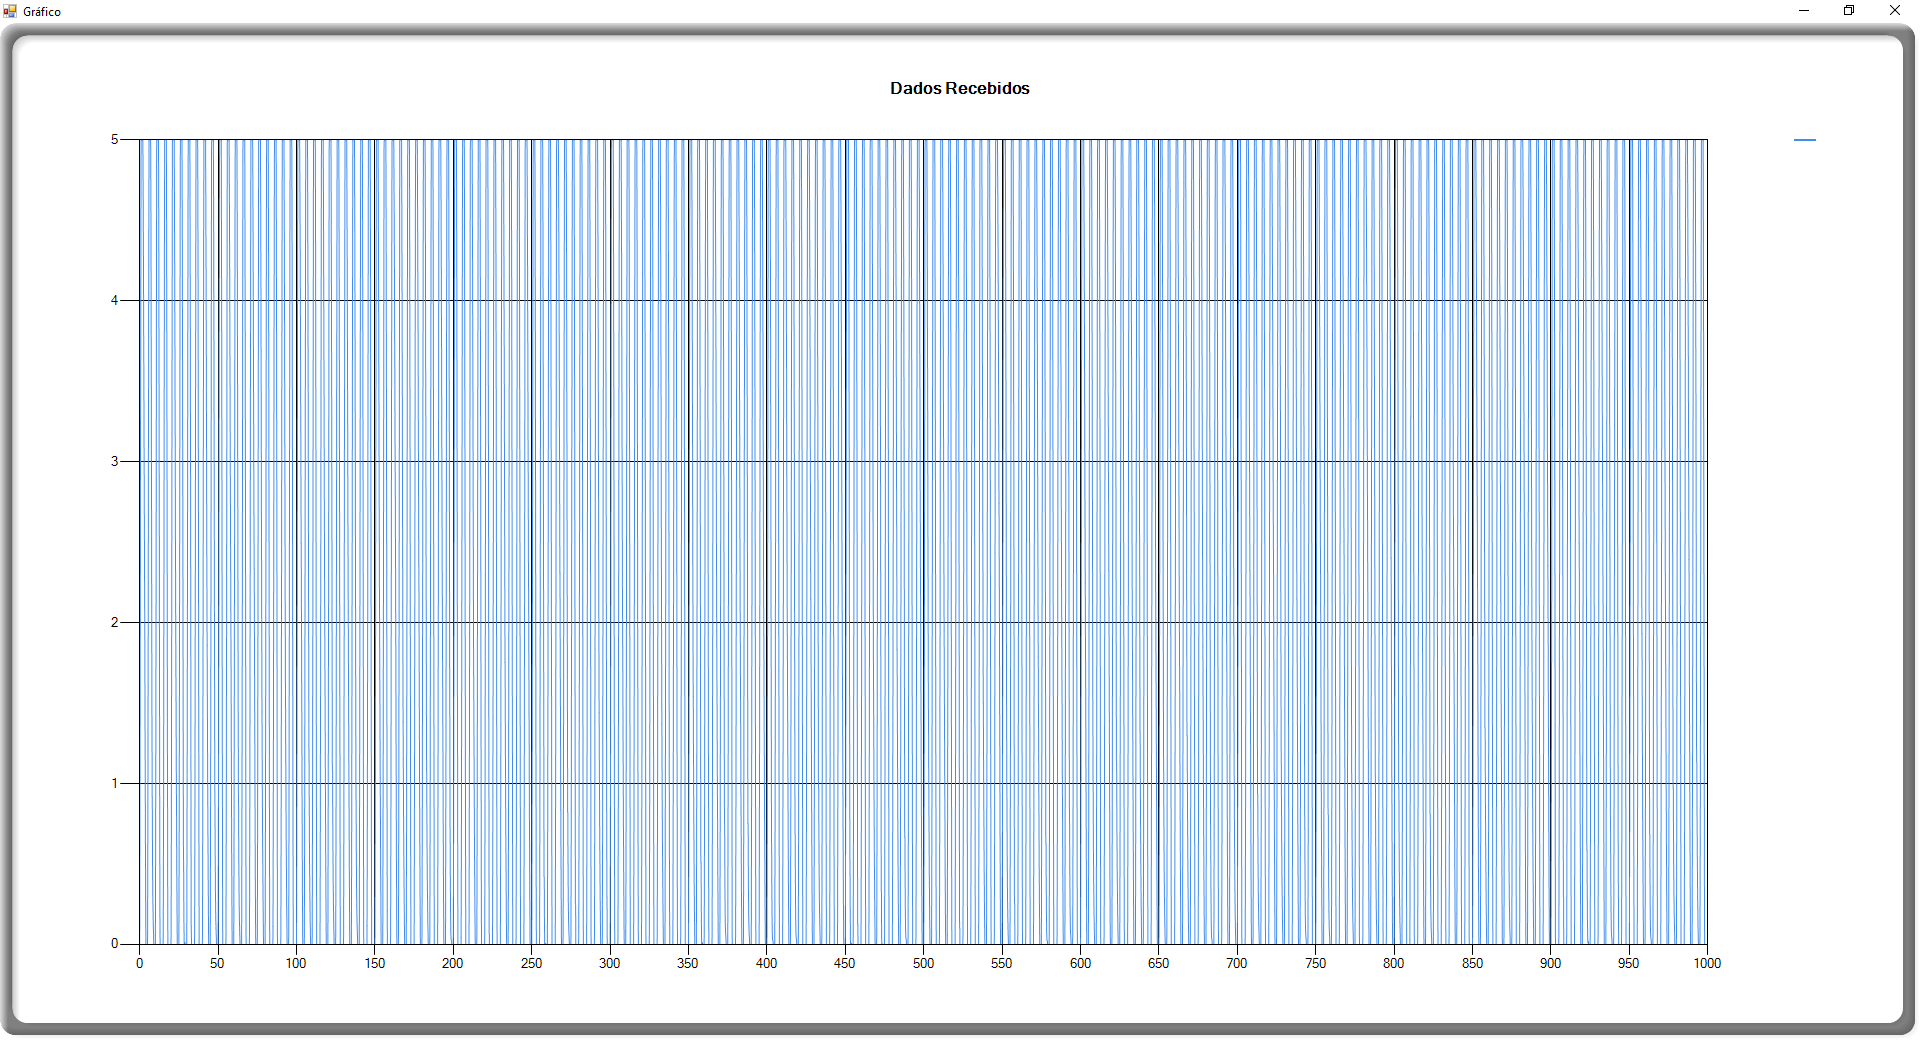
\includegraphics[scale=0.22]{figuras/sinal37}
	}
	\fonte{os autores.}
\end{figure}

\begin{figure}[htb]
	\caption{Software supervisório - Aplicado DFT}
	%	\label{diag:grafico6}
	\borda{
		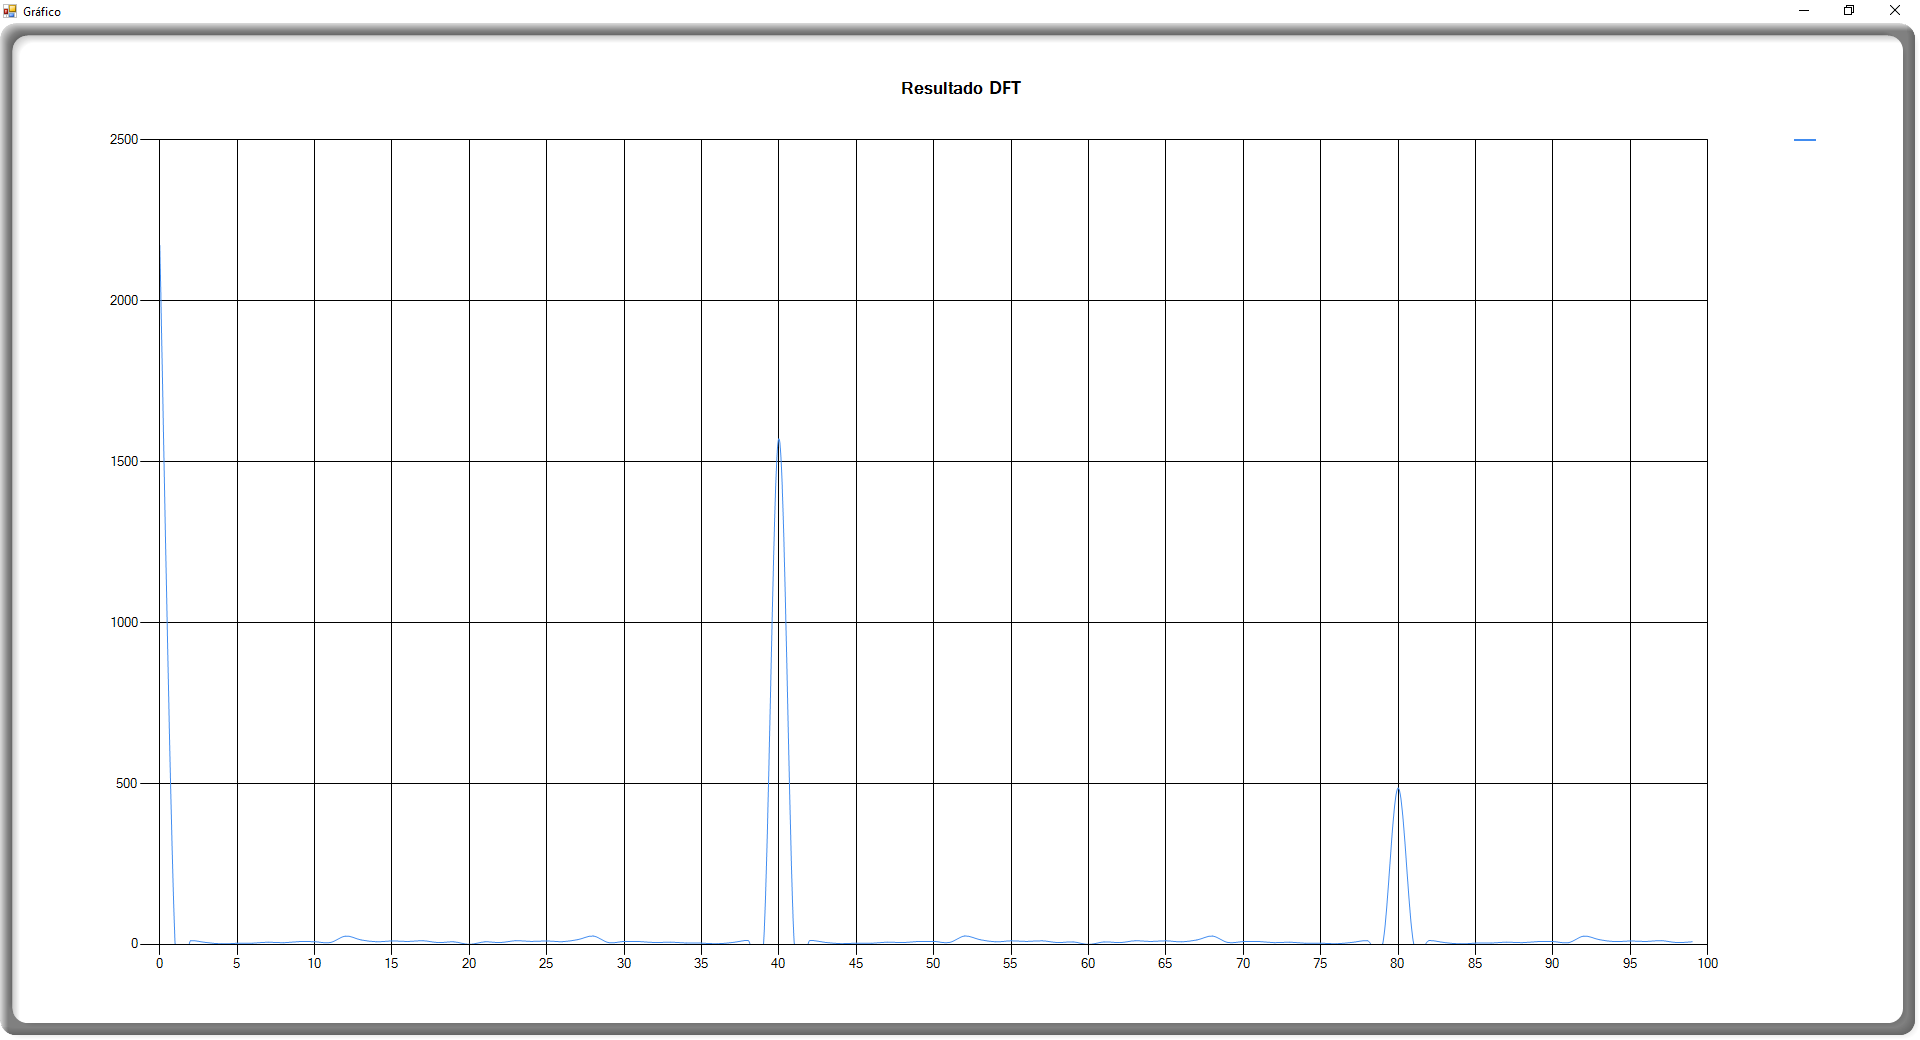
\includegraphics[scale=0.37]{figuras/dft37}
	}
	\fonte{os autores.}
\end{figure}

No segundo teste foi utilizado uma frequência de 67 Hz, podemos visualizar a leitura do sinal na Figura 9 e a DFT na Figura 10.

\begin{figure}[htb]
	\caption{Software supervisório - Entrada sinal}
	%	\label{diag:grafico6}
	\borda{
		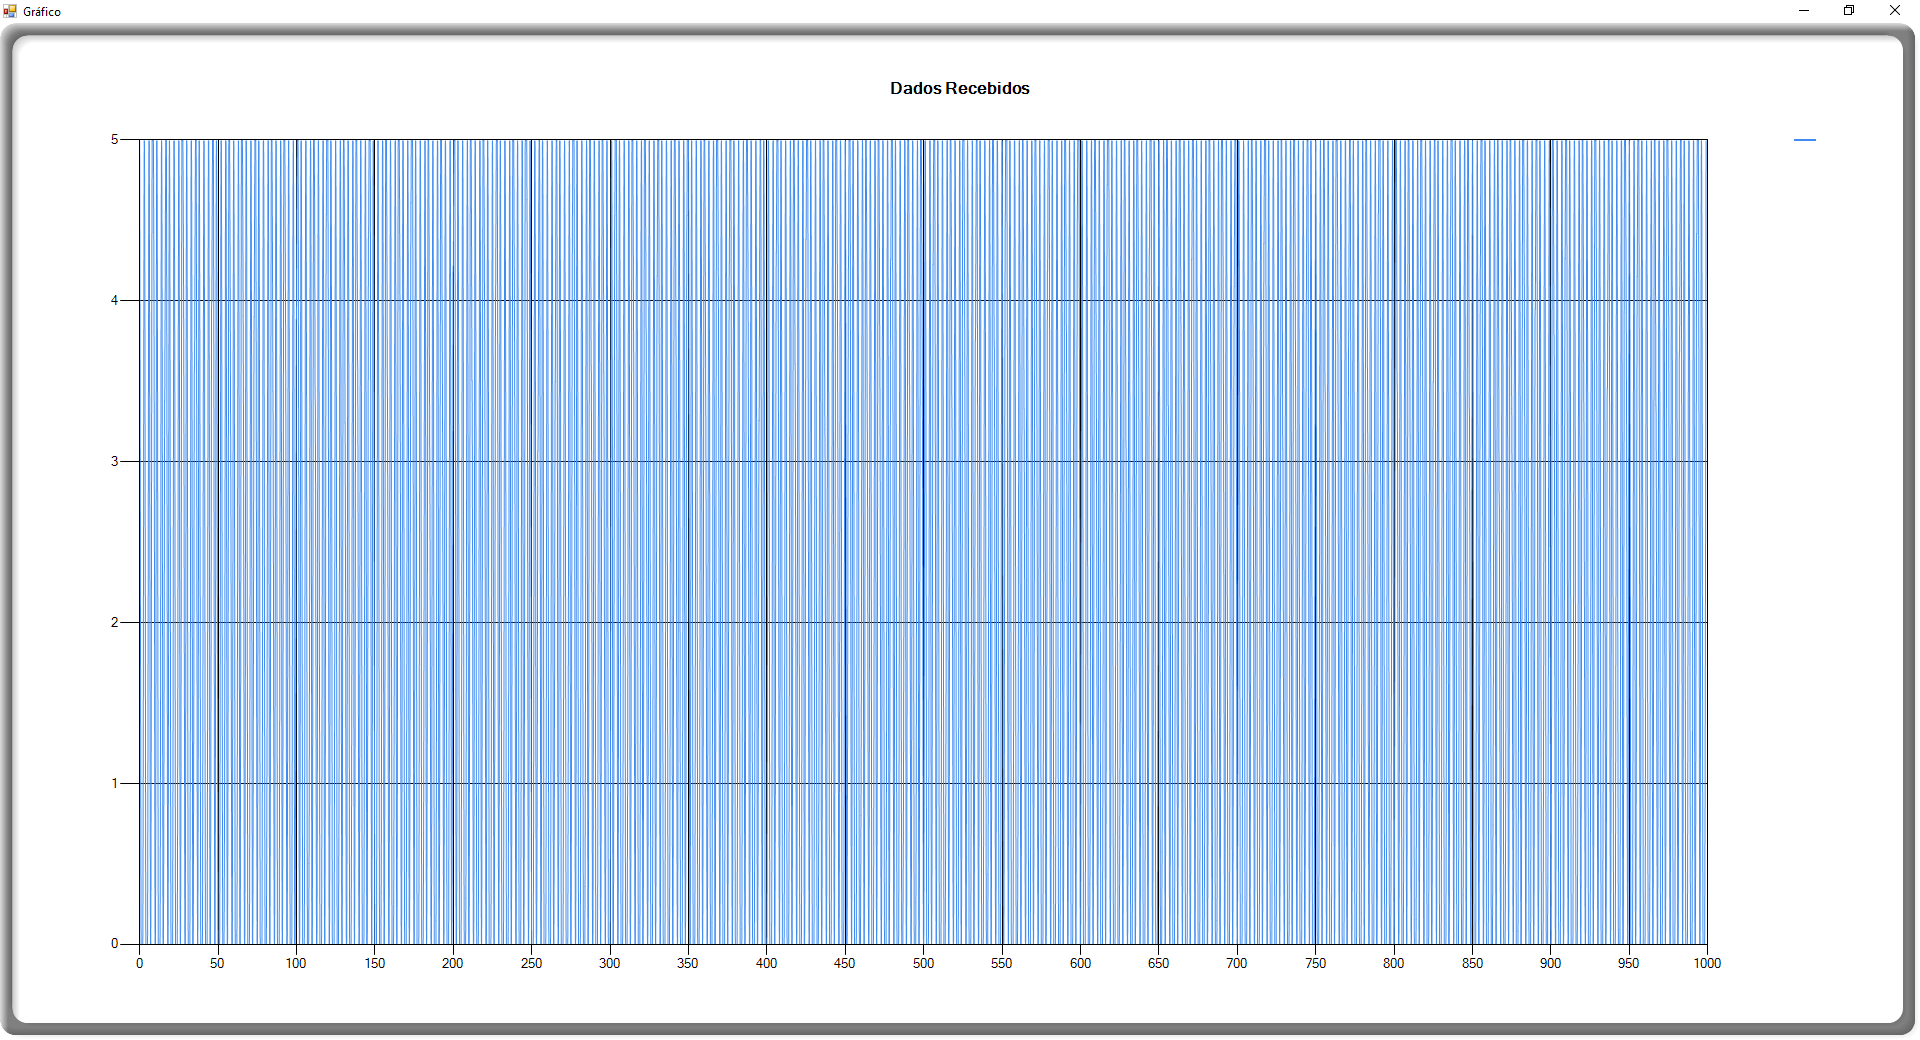
\includegraphics[scale=0.22]{figuras/sinal67}
	}
	\fonte{os autores.}
\end{figure}

\begin{figure}[htb]
	\caption{Software supervisório - Aplicado DFT}
	%	\label{diag:grafico6}
	\borda{
		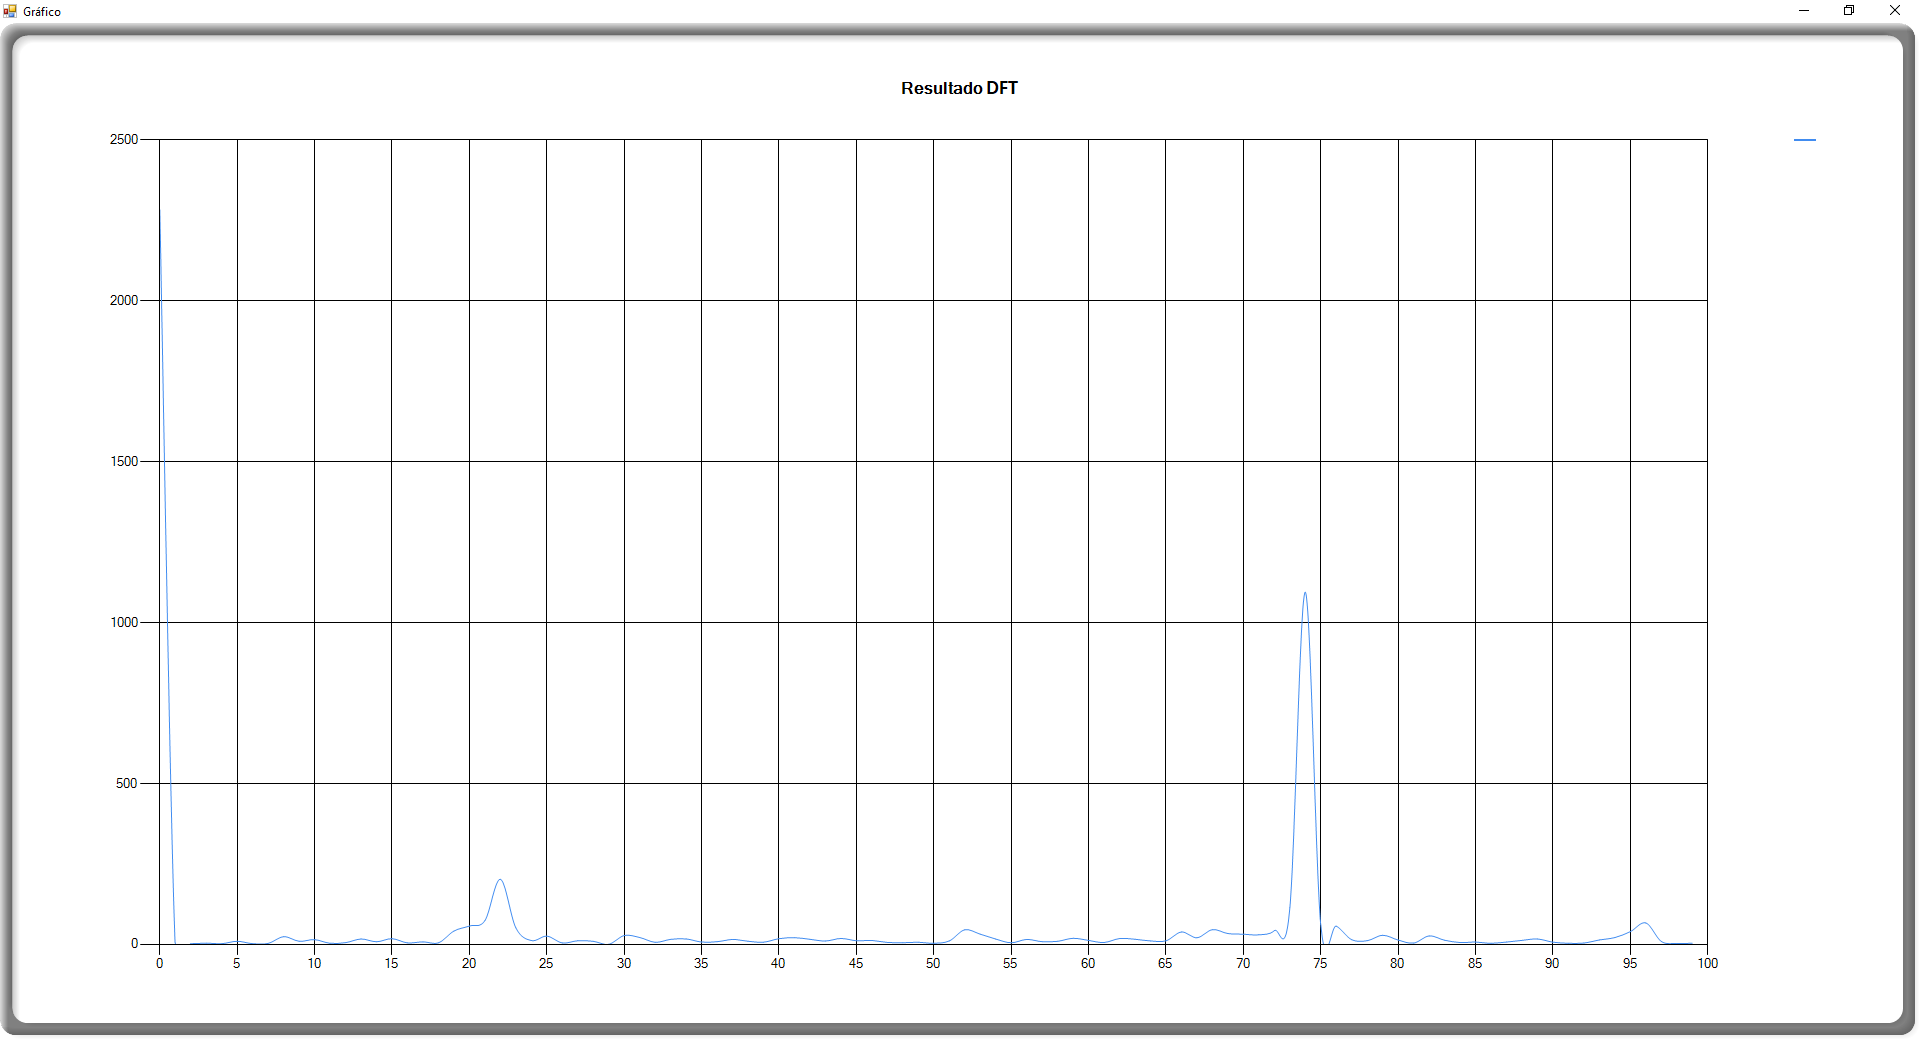
\includegraphics[scale=0.37]{figuras/dft67}
	}
	\fonte{os autores.}
\end{figure}

Nas figuras podemos verificar que na DFT houve uma pequena oscilação na frequência do sinal, foram realizado testes com o osciloscópio na saída do hardware e foi constatado que a frequência do mesmo estava correta. Presume-se que pode estar ocorrendo alguma inconsistência no cálculo da DFT no software gerando este deslocamento na frequência do sinal. 

